\documentclass[11pt, openright]{book}

    % Cover Variables
    \newcommand{\ctoptitle}{}
    \newcommand{\ctitle}{Title}
    \newcommand{\cautor}{Author}
    \newcommand{\cdate}{day.month.year}
    \newcommand{\sectittle}{Second Title}


    % Header Variables
        \newcommand{\headRE}{Main Topic}
        \newcommand{\headLE}{\emph{\rightmark}}
        \newcommand{\footRE}{\cautor $-$ \cdate}
        \newcommand{\footLE}{\emph{\thepage}}

    % TOC Variables
        \newcommand{\toctitle}{Table of Content}
        
        \newcommand{\tocchapter}{Chapter}
        \newcommand{\toccount}{3}
  
    % Chapter Variables
        \newcommand{\chvar}{Chapter -}

\usepackage[a4paper, total={16cm, 22.125cm}]{geometry}

% Page Style
\usepackage[]{environ}
% Cover Page 
\usepackage{tikz}
\makeatletter
\def\parsecomma#1,#2\endparsecomma{\def\page@x{#1}\def\page@y{#2}}
\tikzdeclarecoordinatesystem{page}{
    \parsecomma#1\endparsecomma
    \pgfpointanchor{current page}{north east}
    % Save the upper right corner
    \pgf@xc=\pgf@x%
    \pgf@yc=\pgf@y%
    % save the lower left corner
    \pgfpointanchor{current page}{south west}
    \pgf@xb=\pgf@x%
    \pgf@yb=\pgf@y%
    % Transform to the correct placement
    \pgfmathparse{(\pgf@xc-\pgf@xb)/2.*\page@x+(\pgf@xc+\pgf@xb)/2.}
    \expandafter\pgf@x\expandafter=\pgfmathresult pt
    \pgfmathparse{(\pgf@yc-\pgf@yb)/2.*\page@y+(\pgf@yc+\pgf@yb)/2.}
    \expandafter\pgf@y\expandafter=\pgfmathresult pt
}
\makeatother


% Object formatting
\usepackage[12pt]{moresize}
\usepackage[]{anyfontsize}
\usepackage{titlesec}
\usepackage{import}
\usepackage{floatrow}
\usepackage{enumitem}
\usepackage{changepage}
\usepackage[normalem]{ulem}
\usepackage{array}
\newcommand{\ul}[1]{\underline{#1}}

\usepackage[]{chngcntr}
\usepackage{ifthen}
\ifthenelse{\figcountdepth > 1}
  {\counterwithin{figure}{section}\counterwithin{table}{section}}
  {}

\usepackage[format=plain, labelfont=it, textfont=it]{caption}
\makeatletter
\def\@makecaption#1#2{%
    \vskip\abovecaptionskip
    \sbox\@tempboxa{\textit{#1.} #2}

       
   

    \ifdim \wd\@tempboxa >\hsize
        #1. #2\par
    \else
        \global \@minipagefalse
        \hb@xt@\hsize{\hfil\box\@tempboxa\hfil}
    \fi
    \vskip\belowcaptionskip}
\makeatother

\DeclareCaptionFormat{underline}{\uline{#1#2#3}\par}

% Sections
\titleformat{\section}{\fontsize{16}{19.2}\bfseries}{\thesection.}{0.25em}{}
\titleformat{\subsection}{\fontsize{14}{16.8}\bfseries}{\tab\thesubsection.}{0.25em}{}
\titleformat{\subsubsection}{\fontsize{10}{12}}{\uline{\thesubsubsection)\enspace}}{0em}{\uline}





% Geometry

% Typewritting

\setlength{\parskip}{1em}
\setlength{\parindent}{0em}


\newenvironment{items}[3][0pt]
{\def\closesep{#3}
    \vspace{#2}
    \begin{itemize}
        \setlength{\itemsep}{#1}
        \setlength{\topsep}{0pt}
        \setlength{\partopsep}{0pt}}
        {\end{itemize}
    \vspace{\closesep}}

\newenvironment{enum}[3][0pt]
{\defclosesep{#3}
    \vspace{#2}
    \begin{enumerate}
        \setlength{\itemsep}{#1}
        \setlength{\topsep}{0pt}
        \setlength{\partopsep}{0pt}}
        {\end{enumerate}
    \vspace{\closesep}}

\newenvironment{eq}[2]
{\def\closesep{#2}
    \vspace{#1}
    \begin{align*}}
        {\end{align*}
    \vspace{\closesep}}

\newenvironment{lfeq}[2]
{\def\closesep{#2}
    \vspace{#1}
    \begin{flalign*}}
        {\end{flalign*}
    \vspace{\closesep}}
% List Formatting


\NewEnviron{dent}[1]{
    \vspace{-10pt}
    \begin{adjustwidth}{7mm}{}
        \uline{#1}\hspace{2mm}
        \BODY
    \end{adjustwidth}
    \vspace{-10pt}
}


\usepackage[framemethod=tikz]{mdframed}
\newcounter{count_theorem}[section]\setcounter{count_theorem}{0}
\newcommand{\thetheorem}{\arabic{count_theorem}}

\newcounter{count_exercise}[section]\setcounter{count_exercise}{0}
\newcommand{\theexercise}{\arabic{count_exercise}}


\newenvironment{theorem}[1][]{
    \refstepcounter{count_theorem}
    \mdfsetup{
        linecolor=red!30,
        innerbottommargin=10pt,
        linewidth=2pt,
        topline=false,
        bottomline=false,
        rightline=false,
        shadow=true,
        shadowsize=4.5pt,
        frametitlerule=false,
        apptotikzsetting={
                \tikzset{
                    mdfbackground/.append style={
                            left color=red!8,right color=red!3
                        }
                }
            }
    }
    \begin{mdframed}[]\relax
        \ifstrempty{#1}
        {\textbf{Theorem~\thetheorem.} }
        {\textbf{Theorem~\thetheorem.~#1} }
        }
        {\end{mdframed}\vspace{-10pt}
}

\newenvironment{note}{
    \mdfsetup{innertopmargin=5pt,
        linecolor=gray!30,
        linewidth=2pt,
        topline=false,
        bottomline=false,
        rightline=false,
        frametitleaboveskip=0pt,
        shadow=false,
        shadowsize=4pt,
        frametitlerule=false,
        apptotikzsetting={
                \tikzset{
                    mdfbackground/.append style={
                            left color=gray!8,right color=gray!3
                        }
                }
            }
    }
    \begin{mdframed}[]\relax
        \textbf{Note. }
        }
        {\end{mdframed}\vspace{-10pt}
}

\newenvironment{example}{
    \mdfsetup{innertopmargin=5pt,
        linecolor=green!30,
        linewidth=2pt,
        topline=false,
        bottomline=false,
        rightline=false,
        frametitleaboveskip=0pt,
        shadow=false,
        shadowsize=4pt,
        frametitlerule=false,
        apptotikzsetting={
                \tikzset{
                    mdfbackground/.append style={
                            left color=green!7,right color=green!2
                        },
                    mdfframetitlebackground/.append style={
                            left color=green!7,right color=green!2
                        }
                }
            }
    }
    \begin{mdframed}[]\relax
        \textbf{Example. }
        }
        {\end{mdframed}\vspace{-10pt}
}


\usetikzlibrary{calc,arrows}

\tikzset{
    excursus arrow/.style={%
            line width=2pt,
            draw=gray!40,
            rounded corners=2ex,
        },
    excursus head/.style={
            fill=white,
            font=\bfseries\sffamily,
            text=gray!80,
            anchor=base west,
        },
    excursus line/.style={%
            line width=2pt,
            draw=gray!40,
            rounded corners=2ex,
        }
}

\newenvironment{exercise}[1][]{%
    \refstepcounter{count_exercise}
    \mdfsetup{
        singleextra={
                \path let \p1=(P), \p2=(O) in (\x2,\y1) coordinate (Q);
                \path let \p1=(Q), \p2=(O) in (\x1,{(\y1-\y2)/2}) coordinate (M);
                \path [excursus line] ($(O)+(5em,0ex)$) -| (M) |- ($(Q)+(20em,0ex)$);
                \node [excursus head] at ($(Q)+(2.5em,-0.75pt)$) {\ifstrempty{#1}{Exercise \theexercise}{Exercise \theexercise:~#1}};},
        firstextra={
                \path let \p1=(P), \p2=(O) in (\x2,\y1) coordinate (Q);
                \path [excursus arrow,-to] (O) |- ($(Q)+(12em,0ex)$) .. controls +(0:16em) and +(185:6em) .. ++(23em,2ex);},
        middlelinewidth=2.5em,middlelinecolor=white,
        hidealllines=true,topline=true,
        innertopmargin=0.5ex,
        innerbottommargin=2.5ex,
        innerrightmargin=2pt,
        innerleftmargin=2ex,
        skipabove=0.87\baselineskip,
        skipbelow=0.62\baselineskip,
    }
    \begin{mdframed}[]\relax}
        {\end{mdframed}\vspace{-10pt}
}

% Functions and Data Plotting
\usepackage{subfig,wrapfig,adjustbox,multirow}


% Plotting Style
\usepackage{graphicx,pgfplots}
\usetikzlibrary{arrows}
\usetikzlibrary {patterns,patterns.meta}
\usepgfplotslibrary{fillbetween}
\pgfplotsset{compat=1.18}

\usepgfplotslibrary{units}
% Logarithmic Scale
\pgfplotsset{
    log x ticks with fixed point/.style={
            xticklabel={
                    \pgfkeys{/pgf/fpu=true}
                    \pgfmathparse{exp(\tick)}%
                    \pgfmathprintnumber[fixed relative, precision=3]{\pgfmathresult}
                    \pgfkeys{/pgf/fpu=false}
                }
        }
}


% Mathematics

% Formatting
\usepackage{amsmath}
\usepackage{esvect}
\usepackage{amsfonts}
\usepackage{tasks,environ}
\usepackage{xargs}
\usepackage{esint}
\usepackage[]{listings}


\usepackage[english]{babel}
\usepackage{amsthm}
%\newtheorem{theorem}{Theorem}
%\newtheorem{proof}{Proof}



%Custom Shortcuts
\newcommand{\eqi}{\Leftrightarrow}
\newcommand{\lr}[1]{\left( #1 \right)}
\newcommand{\limit}[1]{\displaystyle{\lim_{#1}}}
\newcommand{\tab}{\hspace*{7mm}}
\newcommand{\ds}[1]{\displaystyle{#1}}
\newcommand{\floor}[1]{\lfloor #1 \rfloor}
\newcommand{\R}{\mathbb{R}}
\newcommand{\N}{\mathbb{N}}
\newcommand{\Z}{\mathbb{Z}}
\newcommand{\C}{\mathbb{C}}
\newcommand{\K}{\mathbb{K}}
\newcommand{\F}{\mathcal{F}}
\newcommand{\M}{\mathcal{M}}
\renewcommand{\l}{\lambda}
\newcommand{\seg}[1]{\overline{\rm {#1}}}
\newcommand{\Int}{\int\limits}
\newcommand{\ex}{\tab \uline{Example :}\hspace{0.2cm} }
\newcommand{\vard}{\partial}
\newcommand{\Q}{\mathcal{Q}}
\newcommand{\Vect}{\operatorname{Vect}}
\newcommand{\rg}{\operatorname{rg}}
\renewcommand{\dim}{\operatorname{dim}}
\renewcommand{\Re}{\operatorname{Re}}
\renewcommand{\Im}{\operatorname{Im}}
\renewcommand{\P}{\mathcal{P}}
\newcommand{\blr}[1]{\left\{#1\right\}}
\newcommand{\linecenter}[1]{\par\vspace{2mm} \centerline{#1}\par\vspace{-2mm}}
\newcommand{\dd}{\textrm{d}}
\newcommand{\supp}{\operatorname{Supp}}
\renewcommand{\vec}{\overrightarrow}
\renewcommand{\epsilon}{\varepsilon}

% Matrix Configurations

\makeatletter
\renewcommand*\env@matrix[1][*\c@MaxMatrixCols c]{%
    \hskip -\arraycolsep
    \let\@ifnextchar\new@ifnextchar
    \array{#1}}
\makeatother


% Colors
\usepackage{xcolor}
\newcommand{\blu}{\color{blue}}
\newcommand{\Red}{\color{red}}
\newcommand{\blac}{\color{black}}

\newcommand{\red}[1]{\textcolor{red}{#1}}

\usepackage{xcolor,xspace}
\usepackage{breqn}


% Headings  
\usepackage[Glenn]{fncychap}
\ChNumVar{\fontsize{40}{42}}
\ChTitleVar{\Large\sc}
\ChNameVar{\Large\sc}
\setlength\headheight{14.5pt}
\renewcommand\FmN[1]{\chvar}



\usepackage{fancyhdr}
\usepackage{ragged2e}

% Header & Footers
\renewcommand{\chaptermark}[1]{\markboth{#1}{#1}}
\renewcommand{\sectionmark}[1]{
    \markright{ #1}
}
\pagestyle{fancy}
\fancyhf{}
\fancyhead[LE,RO]{\headLE}
\fancyhead[RE,LO]{\headRE}
\fancyfoot[LE,RO]{\footLE}
\fancyfoot[RE,LO]{\footRE}
\renewcommand{\headrulewidth}{0.5pt}
\fancyheadoffset{1cm}

\fancypagestyle{plain}{%
    \fancyhf{} % clear all header and footer fields
    \fancyfoot[LE, RO]{\footLE}
    \renewcommand{\headrulewidth}{0pt}
    \renewcommand{\footrulewidth}{0pt}}


\fancypagestyle{nohead}{%
    \fancyhf{} % clear all header 
    \fancyfoot[LE, RO]{\footLE}
    \fancyfoot[LO, RE]{\footRE}}

    \fancypagestyle{head}{%
    \fancyhf{} % clear all header 
    \fancyhead[LE,RO]{\headLE}
\fancyhead[RE,LO]{\headRE}
\renewcommand{\headrulewidth}{0.5pt}
\fancyheadoffset{1cm}
    }


\fancypagestyle{bib}{%
    \fancyhf{} % clear all header and footer fields
    \fancyhead[CE, CO]{}
    \fancyfoot[LE, RO]{\footLE}
    \fancyfoot[LO, RE]{Bibliographie}}

% Table of Contents

\renewcommand*\thechapter{\arabic{chapter}} %Usually Roman
\renewcommand*\thesection{\arabic{section}}
\renewcommand*\thesubsubsection{\thesubsection.\alph{subsubsection}}
\makeatletter
\@removefromreset{section}{chapter}
\makeatother


% Table of Contents

\usepackage{titletoc}
\usepackage{ erewhon,cabin}
\usepackage[linktoc=all]{hyperref}
\renewcommand*\contentsname{\centerline{\toctitle}}

\setcounter{secnumdepth}{3}
\setcounter{tocdepth}{\toccount}

\usepackage[subfigure]{tocloft}
\setlength\cftparskip{0pt}

\usepackage{etoolbox}
\makeatletter
\pretocmd{\chapter}{\addtocontents{toc}{\protect\addvspace{5\p@}}}{}{}
\pretocmd{\section}{\addtocontents{toc}{\protect\addvspace{-10\p@}}}{}{}
\pretocmd{\subsection}{\addtocontents{toc}{\protect\addvspace{1\p@}}}{}{}
\makeatother


% Chapter Style
\titlecontents{chapter}
[11em]
{\bigskip}
{\bfseries\textsc\tocchapter~\textsc\thecontentslabel : \textsc}
{\hspace*{-5.5em}\textbf}
{\titlerule*[1pc]{ }}[\smallskip]

% Section Style
\titlecontents{section}
[0em] % i
{\bigskip\bfseries}
{\fontsize{11}{13.2}\bfseries\uline{\thecontentslabel.\enspace}\uline}
{\hspace*{-4em}\textbf}
{\hspace{0.5pt}\uline{\hspace*{\fill}}\contentspage}

% Subsection Style
\titlecontents{subsection}
[2em] % i
{\smallskip\bfseries}
{\fontsize{10}{12}\bfseries\thecontentslabel.\enspace}
{\hspace*{-4em}}
{\titlerule*[0.5pc]{.}\contentspage}

% Subsubsection Style
\titlecontents{subsubsection}
[4em] % i
{\smallskip}
{\fontsize{10}{12}\thecontentslabel)\enspace}
{\hspace*{-4em}}
{\titlerule*[0.5pc]{.}\contentspage}










    % figure support
    \usepackage{import}
    \usepackage{xifthen}
    \pdfminorversion=7
    \usepackage{pdfpages}
    \usepackage{transparent}
    \newcommand{\incfig}[1]{%
            \def\svgwidth{\columnwidth}
            \import{./figures/}{#1.pdf_tex}
    }

    \pdfsuppresswarningpagegroup=1

    \usepackage{bodegraph}



    \usepackage[]{circuitikz}

\begin{document}
% Spacing
% Section Spacing
\titlespacing\section{0pt}{3pt plus 2pt minus 2pt}{6pt plus 2pt minus 1pt}
\titlespacing\subsection{0pt}{0pt plus 1pt minus 1pt}{0pt plus 3pt minus 1pt}
\titlespacing\subsubsection{0pt}{0pt plus 0pt minus 0pt}{0pt plus 2pt minus 0pt}

\usetikzlibrary{shadows}

\newgeometry{left=2.5cm, width=16cm, bottom=2.5cm, top=2.5cm}






% Cover
% Cover
\definecolor{ccolor1}{RGB}{236,145,143}
\definecolor{ccolor2}{RGB}{131,168,192}
\definecolor{ccolor3}{RGB}{182,227,150}
\definecolor{ccolor4}{RGB}{171,206,145}

\usetikzlibrary{fadings}

\begin{titlepage}
    \newgeometry{top=1cm, width=21cm, bottom=1cm}

    \begin{tikzpicture}[remember picture,overlay,every node/.style={anchor=center}]

        \coordinate (Center) at (page cs: 0,-0.5);
        %F4E Logo
        \begin{scope}[scale = 1.5]
            \foreach \angle in {0,30,...,330} {
                    \filldraw[orange!50!yellow,line width=0.01pt,shift=(Center)] (\angle:3.8637) -- (\angle+30:3.8637) -- (0,0) -- (\angle:3.8637);
                    \draw[white, line width = 7pt,shift=(Center)] (\angle:2cm) arc (\angle-60:\angle:2cm);
                    \draw[white, line width = 7pt,shift=(Center)] (\angle+30:2cm) arc (\angle+90:\angle+30:2cm);
                }
            % Outer delimiter
            \foreach \angle in {15,45,...,345} {
                    \filldraw[white, line width = 7pt,shift=(Center)] (\angle:3.8637cm) arc (\angle-15:\angle+45:2cm) arc (\angle+15:\angle-15:2cm) arc (\angle+45:\angle+15:2cm);
                }
            % Inner delimiter
            \foreach \angle in {15,45,...,345} {
                    \filldraw[white, line width = 7pt,shift=(Center)] (\angle:1.0353cm) arc (\angle-75:\angle-45:2cm) arc (\angle+75:\angle+105:2cm) -- (0,0) -- (\angle:1.0353cm);
                }
            % Stars
            \foreach \angle in {0,30,...,330} {
                    \fill[orange!50!yellow,shift=(Center)] (\angle:1.03527cm) -- ++ (231:0.175) -- ++ (33:0.35) -- ++ (177:0.35) -- ++ (321:0.35) -- ++ (105:0.35) -- ++ (249:0.35) -- ++ (33:0.35);
                }
        \end{scope}

        \node[opacity =0.07, inner sep=0pt, anchor=east] at (current page.east){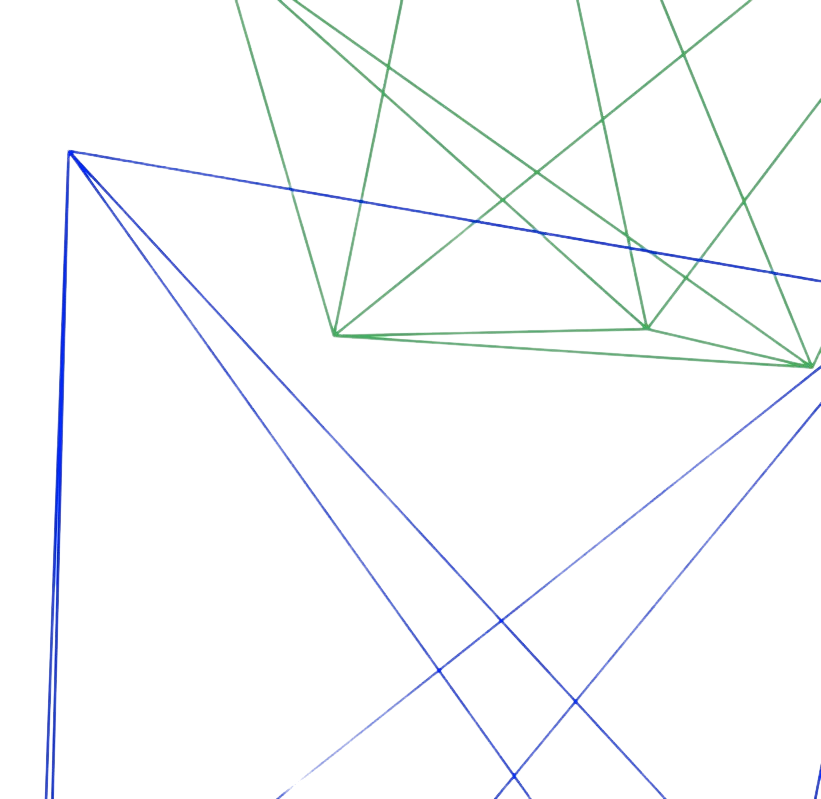
\includegraphics[width=0.5\paperwidth,height=\paperheight]{/root/.config/latex-utils/logos/invert1.png}};

        \node[opacity=0.07,inner sep=0pt, anchor=north west] at (current page.north west){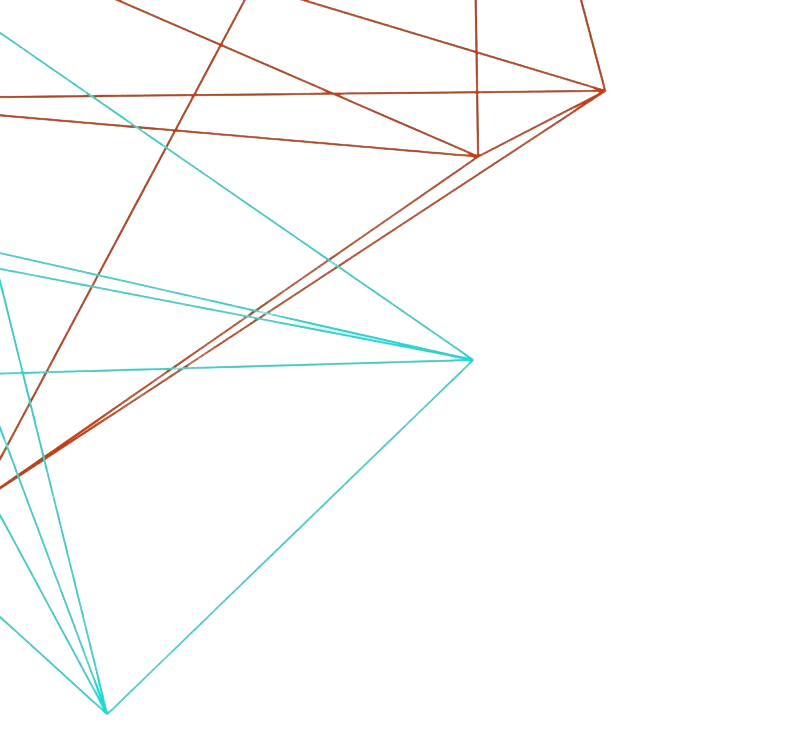
\includegraphics[width=0.5\paperwidth,height=0.5\paperheight]{/root/.config/latex-utils/logos/invert3.png}};




        \node at (page cs:0,0.345) {\Large\textsc{High School Observation and Learning Internship}};
        \node at (page cs:0,0.875) {\Large\bfseries\textsc{Observation Internship}};
        \node at (page cs:0,0.925) {\LARGE\bfseries\textsc{Lycée Français de Barcelone}};

        \node at (page cs:0.5,0) {\Large\textsc{Cyril Lescure - Pedagogical Tutor}};








        %\node[opacity=0.15, inner sep=0pt, anchor=south west] at (current page.south west){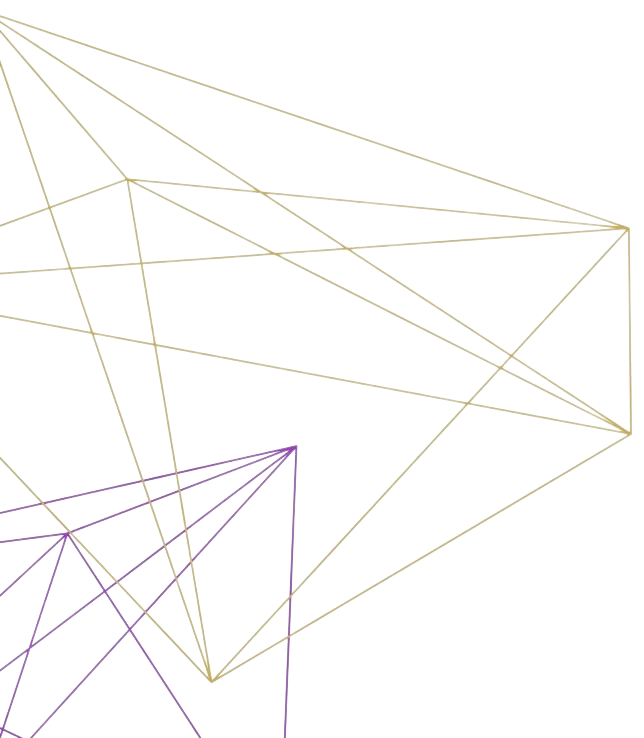
\includegraphics[width=0.5\paperwidth,height=0.5\paperheight]{/root/.config/latex-utils/logos/invert2.png}};

        \node at (page cs:0,0.5) {\fontsize{28}{28.8}\textbf{\ctoptitle}};
        \node at (page cs:0,0.425) {\fontsize{28}{28.8}\textbf{\ctitle}};
        \draw (page cs:0.5,0.375) -- (page cs:-0.5,0.375);
        \node at (page cs:0,0.245) {\LARGE\textsc{\cautor}};
        \node at (page cs:0,0.310) {\Large\textsc{03.06.2019 - 07.06.2019}};


    \end{tikzpicture}
\end{titlepage}


\newgeometry{width=18.625cm, bottom=2cm, top=2cm}

\tikz[remember picture, overlay] \node[opacity=0.3,inner sep=0pt, anchor=north east] at (current page.north east){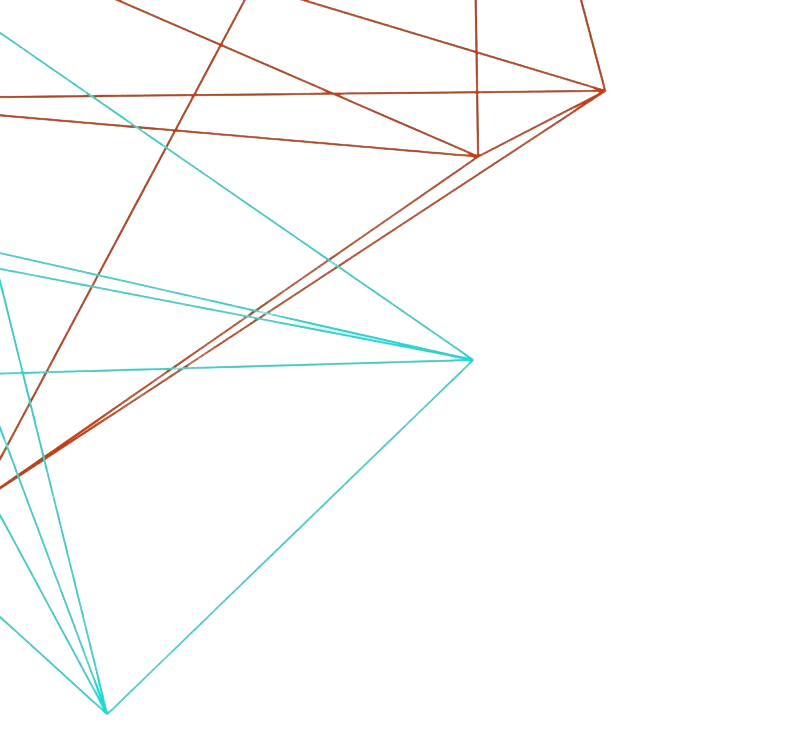
\includegraphics[angle=-90,origin=c,width=0.5\paperheight,height=0.5\paperwidth]{/root/.config/latex-utils/logos/invert3.png}};
\tikz[remember picture,overlay] \node[opacity=0.3,inner sep=0pt, anchor=south east] at (current page.south east){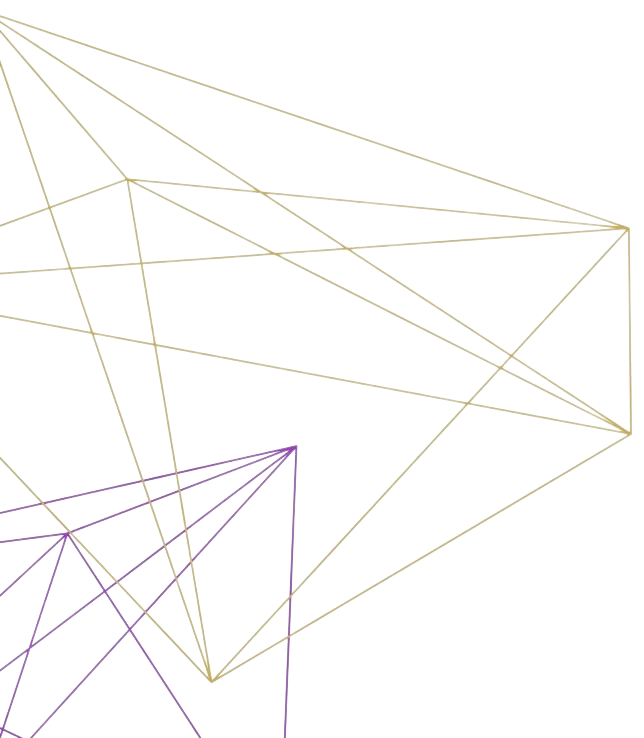
\includegraphics[angle=90,width=0.5\paperwidth,height=0.5\paperheight]{/root/.config/latex-utils/logos/invert2.png}};

\tableofcontents





\newpage

\section{Décomposition en éléments simples}

\subsection{Exercise 1}
Décomposer en éléments simples la fraction rationnelle suivante:
\linecenter{$\ds{F_1(X)= \frac{5X^3+11X^2-2X-2}{X^{4}+2X^3-X^2-2X}}$}


Une fois factorisé en produits de fonctions simples, on procède à retrouver les variable de la décomposition en élement simple de l'expression associé ci-présente, tel que $\ds{A,B,C,D\in \R^{*}}$ :
\linecenter{$\ds{F_1(X)=\frac{A}{X}+\frac{B}{X-1}+\frac{C}{X+1}+\frac{D}{(X+1)^2}}$}

Au niveau du numerateur on obtient alors l'expression suivante:
\linecenter{$\ds{A(X-1)(X+1)^2+BX(X+1)^2+CX(X-1)(X+1)+DX(X-1)}$}

Pour $\ds{X=0}$ on a alors $\ds{A=2}$, pour $\ds{X=1}$ on retrouve $\ds{B=3}$, et pour $\ds{X=-1}$ on a $\ds{D=3}$.




the Bayes theroem is given by:
\begin{equation}
    P(A|B) = \frac{P(B|A)P(A)}{P(B)}
\end{equation}


\newpage



\begin{tikzpicture}[scale=.8]
    \begin{axis}[xmode=log,
            y axis line style={blue},
            y tick label style={blue},
            width=0.6\textwidth, height=0.35\textwidth,
            extra x ticks={50,1e2,500,1e3,2122,1e4},
            extra x tick labels={$50$, ,$500$, ,$2122$, },
            minor x tick num=9,
            xtick pos=bottom,
            xtick align=outside,
            xmin=20,
            xmax=3.1e4,
            ymin=20,
            ymax=100,
            axis y line=left,
            xlabel={Fréquence ($Hz$)},
            x label style={at={(axis description cs:0.5,-0.175)},anchor=north},
            ylabel={Gain de cellule ($dB$)},
            grid=both]
        \addplot [blue,thick,domain=20:3.1e4] {20*ln((2*3.1416*x))/ln(10)};
        \addplot [blue!70,dashed,domain=20:3.1e4] {10*ln(100*((318e-6*2*pi*x)^2+1)/(((75e-6*2*pi*x)^2+1)*((3180e-6*2*pi*x)^2+1)))/ln(10)+20*ln((2*3.1416*x))/ln(10)};
    \end{axis}
    \begin{axis}[xmode=log,
            y axis line style={red},
            y tick label style={red},
            legend style={at={(0.97,0.7)},anchor=north east},
            extra x ticks={50,1e2,500,1e3,2122,1e4},
            extra x tick labels={$50$, ,$500$, ,$2122$, },
            minor x tick num=9,
            grid style={line width=.1pt, draw=gray!10},
            major grid style={line width=.2pt,draw=gray!60},
            xtick pos=bottom,
            xtick align=outside,
            width=0.6\textwidth, height=0.35\textwidth,
            xmin=20,
            xmax=3.1e4,
            ymin=-20,
            ymax=20,
            axis y line=right,
            xlabel={Fréquence ($Hz$)},
            x label style={at={(axis description cs:0.5,-0.175)},anchor=north},
            ylabel={Gain préamp RIAA ($dB$)},
            extra tick style={black},
            grid=both]
        \addplot [blue,thick] coordinates {(20,0) (20,-50)};
        %\addplot [red,thick,domain=20:3.1e4,samples=1000] {20*ln(((318*1e-6*2*pi*x+1))/((3180*1e-6*2*pi*x+1)*(75*1e-6*2*pi*x+1)))/ln(10)};
        \addplot [red,thick,domain=20:3.1e4] {10*ln(100*((318e-6*2*pi*x)^2+1)/(((75e-6*2*pi*x)^2+1)*((3180e-6*2*pi*x)^2+1)))/ln(10)};

        \addplot [red,dashed,domain=20:3.1e4] {20*ln(6309/(2*3.1416*x))/ln(10)};

        \addplot [black, very thin] coordinates {(50,20) (50,-20)};
        \addplot [black, very thin] coordinates {(500,0) (500,-20)};
        \addplot [black, very thin] coordinates {(2122,0) (2122,-20)};

        \addplot [red,thin] coordinates {(20,20) (50,20) (500,0) (2122,0) (20000,-20)};
        \addplot [red,very thick] coordinates {(3.1e4,40) (3.1e4,-40)};
        \addplot [blue,very thick] coordinates {(20,40) (20,-40)};
        \addlegendentry[]{$T\left( \omega \right)$};
        \addlegendentry[]{RIAA};
    \end{axis}
\end{tikzpicture}


$$\mathcal{F}\{\phi(t)\}=\mathcal{F}\left\{-\int e(t) \,dt \right\} \implies \Phi(t)=\frac{1}{j\omega}E\left(t  \right) $$
$$T(\omega)= \frac{\Phi(t)}{E(t)}=\frac{1}{j\omega}$$




\begin{tikzpicture}[scale=.8]
    \begin{axis}[xmode=log,
            y axis line style={blue},
            y tick label style={blue},
            width=0.6\textwidth, height=0.35\textwidth,
            minor x tick num=9,
            xtick pos=bottom,
            xtick align=outside,
            xmin=20,
            xmax=3.1e4,
            ymin=20,
            ymax=100,
            axis y line=left,
            xlabel={Fréquence ($Hz$)},
            x label style={at={(axis description cs:0.5,-0.175)},anchor=north},
            ylabel={Gain de cellule ($dB$)},
            grid=both]
        \addplot [blue,thick,domain=20:3.1e4] {20*ln((2*3.1416*x))/ln(10)};
        \addplot [blue!70,dashed,domain=20:3.1e4] {20*ln(6309/(2*3.1416*x))/ln(10)+20*ln((2*3.1416*x))/ln(10)};
    \end{axis}
    \begin{axis}[xmode=log,
            y axis line style={red},
            y tick label style={red},
            legend style={at={(0.97,0.6)},anchor=north east},
            minor x tick num=9,
            grid style={line width=.1pt, draw=gray!10},
            major grid style={line width=.2pt,draw=gray!60},
            xtick pos=bottom,
            xtick align=outside,
            width=0.6\textwidth, height=0.35\textwidth,
            xmin=20,
            xmax=3.1e4,
            ymin=-20,
            ymax=20,
            axis y line=right,
            xlabel={Fréquence ($Hz$)},
            x label style={at={(axis description cs:0.5,-0.175)},anchor=north},
            ylabel={Gain préamplificateur ($dB$)},
            extra tick style={black},
            grid=both]
        \addplot [blue,thick] coordinates {(20,0) (20,-50)};

        \addplot [red,thick,domain=20:3.1e4] {20*ln(6309/(2*3.1416*x))/ln(10)};

        \addplot [red,very thick] coordinates {(3.1e4,40) (3.1e4,-40)};
        \addplot [blue,very thick] coordinates {(20,40) (20,-40)};
        \addlegendentry[]{$T\left( \omega \right)$};
        \addlegendentry[]{préamp};
    \end{axis}
\end{tikzpicture}


\begin{figure}[ht!]
    \scalebox{.8}{
        \begin{circuitikz}[]
            \draw (0,0) node[op amp] (opamp) {}; %{LT1007};

            \draw (opamp.-) to ++ (-1,0) coordinate (opin) to[short,*-] ++ (0,1.25) coordinate (leftC1) to[C,l=$C_1$] ++ (2,0) coordinate (leftC2) to[C,l=$C_2$] ++ (2,0) coordinate (endC) to [short,-*] (endC |- opamp.out) coordinate (opout) to (opamp.out);

            \draw (opamp.-) ++ (-1,1.25) to[short,-] ++ (0,1.5) coordinate (leftR1) to[R,l=$R_1$] ++ (2,0) coordinate (leftR2) to[R=1<\ohm>,l=$R_2$] ++ (2,0) to[short,-] ++ (0,-1.5);

            \draw (leftC2) to[short,-] (leftR2);

            %\draw (opout) to ++ (0.5,0) node[right] {}; {$V_{out}$};
            %\draw (opin) to ++ (-0.5,0) node[left] {}; {$V_{in}$};
            \draw (opamp.+) to ++ (-0.5,0) to ++ (0,-0.5) node[ground] {};

            \draw[] (opamp.up) to[short, -o] ++ (0,0.25)  ++ (0,0.3) node {$+15V$};
            \draw[] (opamp.down) to[short, -o] ++ (0,-0.25) ++ (0,-0.3) node {$-15V$};

            %Iteration 2

            \draw[] (opin) ++ (-2,0) coordinate (leftR3) to[vR,l=$R_3$] ++ (2,0);
            \draw[dashed] (leftR3) -- ++ (-0.9,0) coordinate (J1);
            \draw (J1) to[short,-o] ++ (-3,0) coordinate (IN) node[above] {$V_{in}$};
            \draw (J1) ++ (-0.5,0) to[short,*-, R,l={\rotatebox[origin=c]{-90}{$R_{in}$}},a={\rotatebox[origin=c]{-90}{$47\,k\Omega$}}] ++ (0,-2) ++ (0,0.4) node[ground] {};
            \draw (J1) ++ (-2.25,0) to[short,*-, C, l={\rotatebox[origin=c]{-90}{$C_{in}$}},a={\rotatebox[origin=c]{-90}{$150\,pF$}}] ++ (0,-2) ++ (0,0.4) node[ground] {};

            \draw (opout) ++ (2,0) coordinate (J2);
            \draw[dashed] (opout) ++ (0.5,0) -- ++ (1,0);
            \draw[] (opout) -- ++ (0.5,0) ++ (1,0) -- ++ (0.5,0);
            \draw (J2) ++ (3.5,-0.5) node[op amp] (opamp2) {};
            \draw (J2) to [short,*-,R,l=$R_5$] ++ (2.25,0);
            \draw (opamp2.-) to[short,*-] ++ (0,1.5) to[R,l=$R_4$] ++ (2.5,0) coordinate(rightR4) to[short,-*] (rightR4 |- opamp2.out);

            \draw (J2) -- ++ (0,3) to[short,-o] ++ (2,0)  node[above] {AUX};
            \draw (J2) ++ (1,3) to[short,*-,R,l={\rotatebox[origin=c]{-90}{$R_{out}$}}, a={\rotatebox[origin=c]{-90}{$47\,k\Omega$}}] ++ (0,-1.75) ++ (0,0.3) node[ground]{};

            \draw (opamp2.+) to ++ (-0.5,0) to ++ (0,-0.5) node[ground] {};
            \draw (opamp2.out) to[short,-o] ++ (2,0) node[above] {Casques};
            \draw (opamp2.up) to[short, -o] ++ (0,0.25)  ++ (0,0.3) node {$+15V$};
            \draw (opamp2.down) to[short, -o] ++ (0,-0.25) ++ (0,-0.3) node {$-15V$};
            \draw (opamp2.out) ++ (1,0) to[short,*-,R,l={\rotatebox[origin=c]{-90}{$R_{out}$}}, a={\rotatebox[origin=c]{-90}{$55\,\Omega$}}] ++ (0,-1.75) ++ (0,0.3) node[ground] {};

        \end{circuitikz}}
\end{figure}

\begin{figure}[ht!]
    \scalebox{.7}{
        \begin{circuitikz}[]
            \draw (0,0) node[op amp] (opamp) {LT1007};

            \draw (opamp.-) to ++ (-1,0) coordinate (opin) to[short,*-] ++ (0,1.75) coordinate (leftC1) to[C,l=$C_1$,a=$3.18\,nF$] ++ (2,0) coordinate (leftC2) to[C,l=$C_2$,a=$886\,pF$] ++ (2,0) coordinate (endC) to [short,-*] (endC |- opamp.out) coordinate (opout) to (opamp.out);

            \draw (opamp.-) ++ (-1,1.25) to[short,-] ++ (0,2.2) coordinate (leftR1) to[R,l=$R_1$,a=$1\,M\Omega$] ++ (2,0) coordinate (leftR2) to[R=1<\ohm>,l=$R_2$,a=$85\,k\Omega$] ++ (2,0) to[short,-] ++ (0,-2.2);

            \draw (leftC2) to[short,-] (leftR2);

            %\draw (opout) to ++ (0.5,0) node[right] {}; {$V_{out}$};
            %\draw (opin) to ++ (-0.5,0) node[left] {}; {$V_{in}$};
            \draw (opamp.+) to ++ (-0.5,0) to ++ (0,-0.5) node[ground] {};

            \draw[] (opamp.up) to[short, -o] ++ (0,0.25)  ++ (0,0.3) node {$+15V$};
            \draw[] (opamp.down) to[short, -o] ++ (0,-0.25) ++ (0,-0.3) node {$-15V$};

            %Iteration 2

            \draw[] (opin) ++ (-2,0) coordinate (leftR3) to[vR,l=$R_3$, a=$1.085\,k\Omega$] ++ (2,0);
            \draw (leftR3) ++ (-1.5,0) node[op amp] (opamp3) {LT1007} ;
            \draw (opamp3.out) to (leftR3);

            \draw (opamp3.+) to[short,-o] ++ (-3,0) coordinate (IN) node[above] {$V_{in}$};
            \draw (opamp3.+) ++ (-0.5,0) to[short,*-, R,l={\rotatebox[origin=c]{-90}{$R_{in}$}},a={\rotatebox[origin=c]{-90}{$47\,k\Omega$}}] ++ (0,-2) ++ (0,0.4) node[ground] {};
            \draw (opamp3.+) ++ (-2.25,0) to[short,*-, C, l={\rotatebox[origin=c]{-90}{$C_{in}$}},a={\rotatebox[origin=c]{-90}{$150\,pF$}}] ++ (0,-2) ++ (0,0.4) node[ground] {};
            \draw (opamp3.-) to ++ (0,1) to ++ (2.5,0) to[short,-*] ++ (0,-1.5);
            \draw[] (opamp3.up) to[short, -o] ++ (0,0.25)  ++ (0,0.3) node {$+15V$};
            \draw[] (opamp3.down) to[short, -o] ++ (0,-0.25) ++ (0,-0.3) node {$-15V$};

            \draw (opout) ++ (2,0) coordinate (J2);
            \draw[] (opout) ++ (0.5,0) -- ++ (1,0);
            \draw[] (opout) -- ++ (0.5,0) ++ (1,0) -- ++ (0.5,0);
            \draw (J2) ++ (3.5,-0.5) node[op amp] (opamp2) {LT1007};
            \draw (J2) to [short,*-,R,l=$R_5$,a=$10\,k\Omega$] ++ (2.25,0);
            \draw (opamp2.-) to[short,*-] ++ (0,2) to[R,l=$R_4$,a=$63.4\,k\Omega$] ++ (2.5,0) coordinate(rightR4) to[short,-*] (rightR4 |- opamp2.out);

            \draw (J2) -- ++ (0,3) to[short,-o] ++ (2,0)  node[above] {AUX};
            \draw (J2) ++ (1,3) to[short,*-,R,l={\rotatebox[origin=c]{-90}{$R_{out}$}}, a={\rotatebox[origin=c]{-90}{$47\,k\Omega$}}] ++ (0,-1.75) ++ (0,0.3) node[ground]{};

            \draw (opamp2.+) to ++ (-0.5,0) to ++ (0,-0.5) node[ground] {};
            \draw (opamp2.up) to[short, -o] ++ (0,0.25)  ++ (0,0.3) node {$+15V$};
            \draw (opamp2.down) to[short, -o] ++ (0,-0.25) ++ (0,-0.3) node {$-15V$};


            \draw (opamp2.out) ++ (2,0) node[buffer,scale=1.5] (opamp4) {\tiny LT1010};
            \draw (opamp2.out) -- (opamp4.in);
            \draw (opamp4.out) to[short,-o] ++ (2,0) node[above] {Casques};
            \draw (opamp4.out) ++ (1,0) to[short,*-,R,l={\rotatebox[origin=c]{-90}{$R_{out}$}}, a={\rotatebox[origin=c]{-90}{$55\,\Omega$}}] ++ (0,-1.75) ++ (0,0.3) node[ground] {};
            \draw (opamp4.out) ++ (-1,0.5) to[short, -o] ++ (0,0.25)  ++ (0,0.3) node {$+15V$};
            \draw (opamp4.out) ++ (-1,-0.5) to[short, -o] ++ (0,-0.25)  ++ (0,-0.3) node {$-15V$};





        \end{circuitikz}}
\end{figure}



\linecenter{$\ds{\boxed{T(s)= \frac{R_1+R_2}{R_3}\cdot\frac{1+s\frac{R_2R_1}{R_1+R_2}(C_1+C_2)}{(1+sR_1C_1)(1+sR_2C_2)}}}$}


\begin{tikzpicture}
    \begin{axis}[xmode=log,
            y axis line style={blue},
            y tick label style={blue},
            width=0.6\textwidth, height=0.35\textwidth,
            minor x tick num=9,
            xtick pos=bottom,
            xtick align=outside,
            xmin=20,
            xmax=3.1e4,
            ymin=20,
            ymax=100,
            axis y line=left,
            xlabel={Fréquence ($Hz$)},
            x label style={at={(axis description cs:0.5,-0.175)},anchor=north},
            ylabel={Gain de cellule ($dB$)},
            grid=both]
        \addplot[blue] table [x expr=\thisrowno{0}, y expr=\thisrowno{1}, col sep=space] {../data/g2.txt};
    \end{axis}
\end{tikzpicture}

\newpage


\begin{tikzpicture}
    \draw (-1.35,0) -- ++ (1,0) ++ (1,0) -- (1.35,0);
    \draw[dashed] (-0.5,0) -- (0.5,0);
    \draw (1.35,0.65) rectangle (3.75,-0.65) ++ (-1.2,0.65) node[align=center] {\small Transducteur\\\small de sortie};
    \draw (-1.35,0.65) rectangle (-3.75,-0.65) ++ (1.2,0.65) node[align=center] {\small Transducteur\\\small d'entrée};
    \draw (3.75,0) -- ++ (0.75,0) ++ (0,-0.75) rectangle ++ (2,1.5) ++ (-1,-0.75) node[] {CNA} ++ (1,0) coordinate (CNA);
    \draw (-3.75,0) -- ++ (-0.75,0) ++ (0,-0.75) rectangle ++ (-2,1.5) ++ (1,-0.75) node[] { CAN} ++ (-1,0) coordinate (CAN) ;
    \node[align=center] at (0,0) {\small Transmission\\\small Optique};

    \draw (CAN) -- ++ (-0.5,0) ++ (0,-0.6) rectangle ++ (-1,1.2) ++ (0.5,-0.6) node[] {\small PGA} ++ (-0.5,0.3) coordinate (PGA);

    \draw (PGA) ++ (-0.75,-0.25) circle (0.5) ++ (0.353,0.353) -- ++ (-0.707,-0.707) ++ (0.707,0) -- ++ (-0.707,0.707);
    \draw (PGA) ++ (-0.75,0) node {\small $+$} ++ (-0.303,-0.25) node {\small $+$};
    \draw (PGA) ++ (0,-0.25)-- ++ (-0.25,0);
    \draw (PGA) ++ (-0.75,0.25) -- ++ (0,0.2) node[above] {$\frac{V_{dd}}{2}$};
    \draw (PGA) ++ (-1.25,-0.25) to[short,-o] ++ (-0.5,0) node[above] {$V_{in}$};
    \draw (CNA) to [short,-o] ++ (0.5,0) node[above] {$V_{out}$};



\end{tikzpicture}



\begin{circuitikz}
    \tikzset{
        mux4/.pic = {

                % frame
                \draw[pic actions,thick] (0, -0.83) coordinate (-SW) -- ++(30 : 0.66)
                coordinate (-SE) -- ++(90 : 1) coordinate (-NE) -- ++(150 : 0.66)
                coordinate (-NW) -- cycle;

                % output
                \coordinate (-output) at ($(-SE)!0.5!(-NE)$);

                % select
                \coordinate (-sel) at ($(-SW)!0.5!(-SE)$);

                % input
                \pgfmathsetmacro{\ymin}{-0.5}
                \pgfmathsetmacro{\ymax}{0.5}
                \foreach \i in {0,1,2,3} {
                        \pgfmathsetmacro{\y}{\ymax - (\ymax - \ymin) * \i/3.};
                        \coordinate (-\i) at (0,\y);
                    }
            },
        mux2/.pic = {

                % frame
                \draw[pic actions,thick] (0, -0.58) coordinate (-SW) -- ++(30 : 0.66)
                coordinate (-SE) -- ++(90 : 0.5) coordinate (-NE) -- ++(150 : 0.66)
                coordinate (-NW) -- cycle;

                % output
                \coordinate (-output) at ($(-SE)!0.5!(-NE)$);

                % select
                \coordinate (-seld) at ($(-SW)!0.5!(-SE)$);
                \coordinate (-selu) at ($(-NW)!0.5!(-NE)$);

                % input
                \pgfmathsetmacro{\ymin}{-0.33}
                \pgfmathsetmacro{\ymax}{0.33}
                \foreach \i in {0,1} {
                        \pgfmathsetmacro{\y}{\ymax - (\ymax - \ymin) * \i/1.};
                        \coordinate (-\i) at (0,\y);
                    }
            }
    }
    \ctikzset{bipoles/resistor/height=0.15}
    \ctikzset{bipoles/resistor/width=0.5}
    \ctikzset{amplifiers/scale=0.65}
    \pic (mux) at (0,0) {mux4};
    \foreach \i/\lbl in {0/CT\_BLOCK,1/AGND,2/Vss,3/SC\_BLOCK} {
            \draw (mux-\i) -- ++ (-0.5,0) node[left] {\scriptsize \lbl};
        }

    \draw (mux-sel) |- ++ (-0.786,-0.33) node[left] {\scriptsize Reference};


    \pic[rotate=180] (mux21) at (1.33,1.75) {mux2};
    \pic (mux22) at (3.75,1.75) {mux2};

    %2,0.25
    \draw (mux-output) -- ++ (0.5,0) to[R,l=$R_a$] ++ (1,0) to[short,-*] ++ (0.25,0) coordinate (RaRb) -| ++ (0.75,0.25) to[R,l=$R_b$] ++ (0,1) to[short,-*] ++ (0,0.83) coordinate (dot);

    \draw (mux22-1) -- (mux21-0) (mux22-0) -- (mux21-1);
    \draw (RaRb) to[short,-*] ++ (0,1.41);

    \node[op amp] (opamp) at (1.5,3) {};
    \draw (opamp.+) -- ++ (-0.25,0) |- (mux21-output);
    \draw (opamp.out) -| (dot);
    \draw (opamp.-) -- ++ (-1,0) node[left] {\scriptsize Input};

    \draw (mux22-output) -| ++ (0.25,-0.75) to[short,-o] ++ (0.25,0) coordinate (sw) ++ (0.5,0) to[short,o-] ++ (0.5,0)  ++ (0,0.15)node[right] {\scriptsize Analog};
    \node at (6.3,0.85) {\scriptsize Bus Out};
    \draw (sw) ++ (0,-0.06) -- ++ (0.5,0.25);
    \draw (mux22-output) -- ++ (1.5,0) node[right] {\scriptsize Output};
    \draw (mux22-output) ++ (0.75,-1) |- ++ (0.75,-0.5) ++ (0,0.15) node[right] {\scriptsize Analog};
    \draw (mux22-output) ++ (1.5,-1.5) ++ (0.4,-0.15) node[right] {\scriptsize Bus};

    \draw (mux22-seld) to[short,-*] ++ (0,-2) coordinate (down);
    \draw (mux21-selu) |- (down) -- ++ (1.83,0) node[right] {\scriptsize Gain};

\end{circuitikz}


\begin{tikzpicture}
    \begin{axis}[xmode=log,
            width=0.6\textwidth, height=0.35\textwidth,
            minor x tick num=9,
            xtick pos=bottom,
            xtick align=outside,
            xmin=20,
            xmax=1e5,
            ymin=-40,
            ymax=20,
            xlabel={Fréquence ($Hz$)},
            x label style={at={(axis description cs:0.5,-0.175)},anchor=north},
            ylabel={Gain ($dB$)},
            grid=both]
        \addplot[blue,mark=+,draw=none] table [x expr=\thisrowno{0}, y expr=20*ln(\thisrowno{1}/0.5)/ln(10), col sep=space] {../data/Bodecirc.txt};
        \draw[thin,blue] (axis cs: 20,18.75) -- (axis cs: 1e5,18.75);
        \draw[thin,blue,dashed] (axis cs: 20,15.75) -- (axis cs: 1.6e4,15.75);
        \draw[thin,blue,dashed] (axis cs: 16e3,15.75) -- (axis cs: 16e3,-40);
        \node[blue] at (axis cs: 1e2,11) {$15.75\,dB$};
        \node[blue] at (axis cs: 7e3,-30) {$16\,kHz$};


    \end{axis}
\end{tikzpicture}



\begin{tikzpicture}
    \begin{axis}[
            width=0.6\textwidth, height=0.35\textwidth,
            minor x tick num=4,
            xtick pos=bottom,
            xtick align=outside,
            xmin=0,
            xmax=23,
            ymin=-80,
            ymax=10,
            xlabel={Fréquence ($kHz$)},
            ylabel={Puissance($dBm$)},
            grid=both]
        \addplot[blue] table [x expr=\thisrowno{0}, y expr=\thisrowno{1}, col sep=space] {../data/FTALL.txt};
        \addlegendentry[]{FT Output};
        \draw [red, thick] (axis cs: 0, -46) -- (axis cs: 23, -46);
        \draw [red, thick] (axis cs: 0,-3) -- (axis cs: 23, -3);
        \node at (axis cs: 3,-42) {\textcolor{red}{\scriptsize$-46\,dBm$}};
        \node at (axis cs: 3,2) {\textcolor{red}{\scriptsize$-3\,dBm$}};
        \node at (axis cs: 16,-15) {\textcolor{red}{ $SNR=43\,dB$}};

    \end{axis}
\end{tikzpicture}

\begin{figure}[ht!]
    \begin{tikzpicture}
        \begin{axis}[
                grid=both,
                minor x tick num=1,
                ytick={-1000,-500,0,500,1000},
                yticklabels={-1,-0.5,0,0.5,1},
                width=0.8\textwidth, height=0.4\textwidth,
                xlabel={Temps ($ms$)},
                %ytick={-75,-50,-25,0,25,50,75},
                ylabel={Amplitude ($V$)},
                xmin=0,
                xmax=100,
                ymin=-1500,
                ymax=1500,
                legend pos=south east,
            ]

            \addplot [blue] table [x expr=\thisrowno{0}, y expr=\thisrowno{1}*1e3, col sep=space] {../data/Soundout.txt};
            \addlegendentry[]{$V_{out}$};
            \draw [red, thick] (axis cs: 0, -1000) -- (axis cs: 100, -1000);
            \draw [red, thick] (axis cs: 0, 1000) -- (axis cs: 100, 1000);
            \node at (axis cs: 20,1230) {\textcolor{red}{\scriptsize$V_{cc}^{max}=2V$}};
        \end{axis}
    \end{tikzpicture}
\end{figure}

test



\end{document}